\documentclass{standalone}
\usepackage{tikz}
\usetikzlibrary{patterns, positioning}
\usepackage[sfdefault]{ClearSans} %% option 'sfdefault' activates Clear Sans as the default text font
\usepackage[T1]{fontenc}

\begin{document}
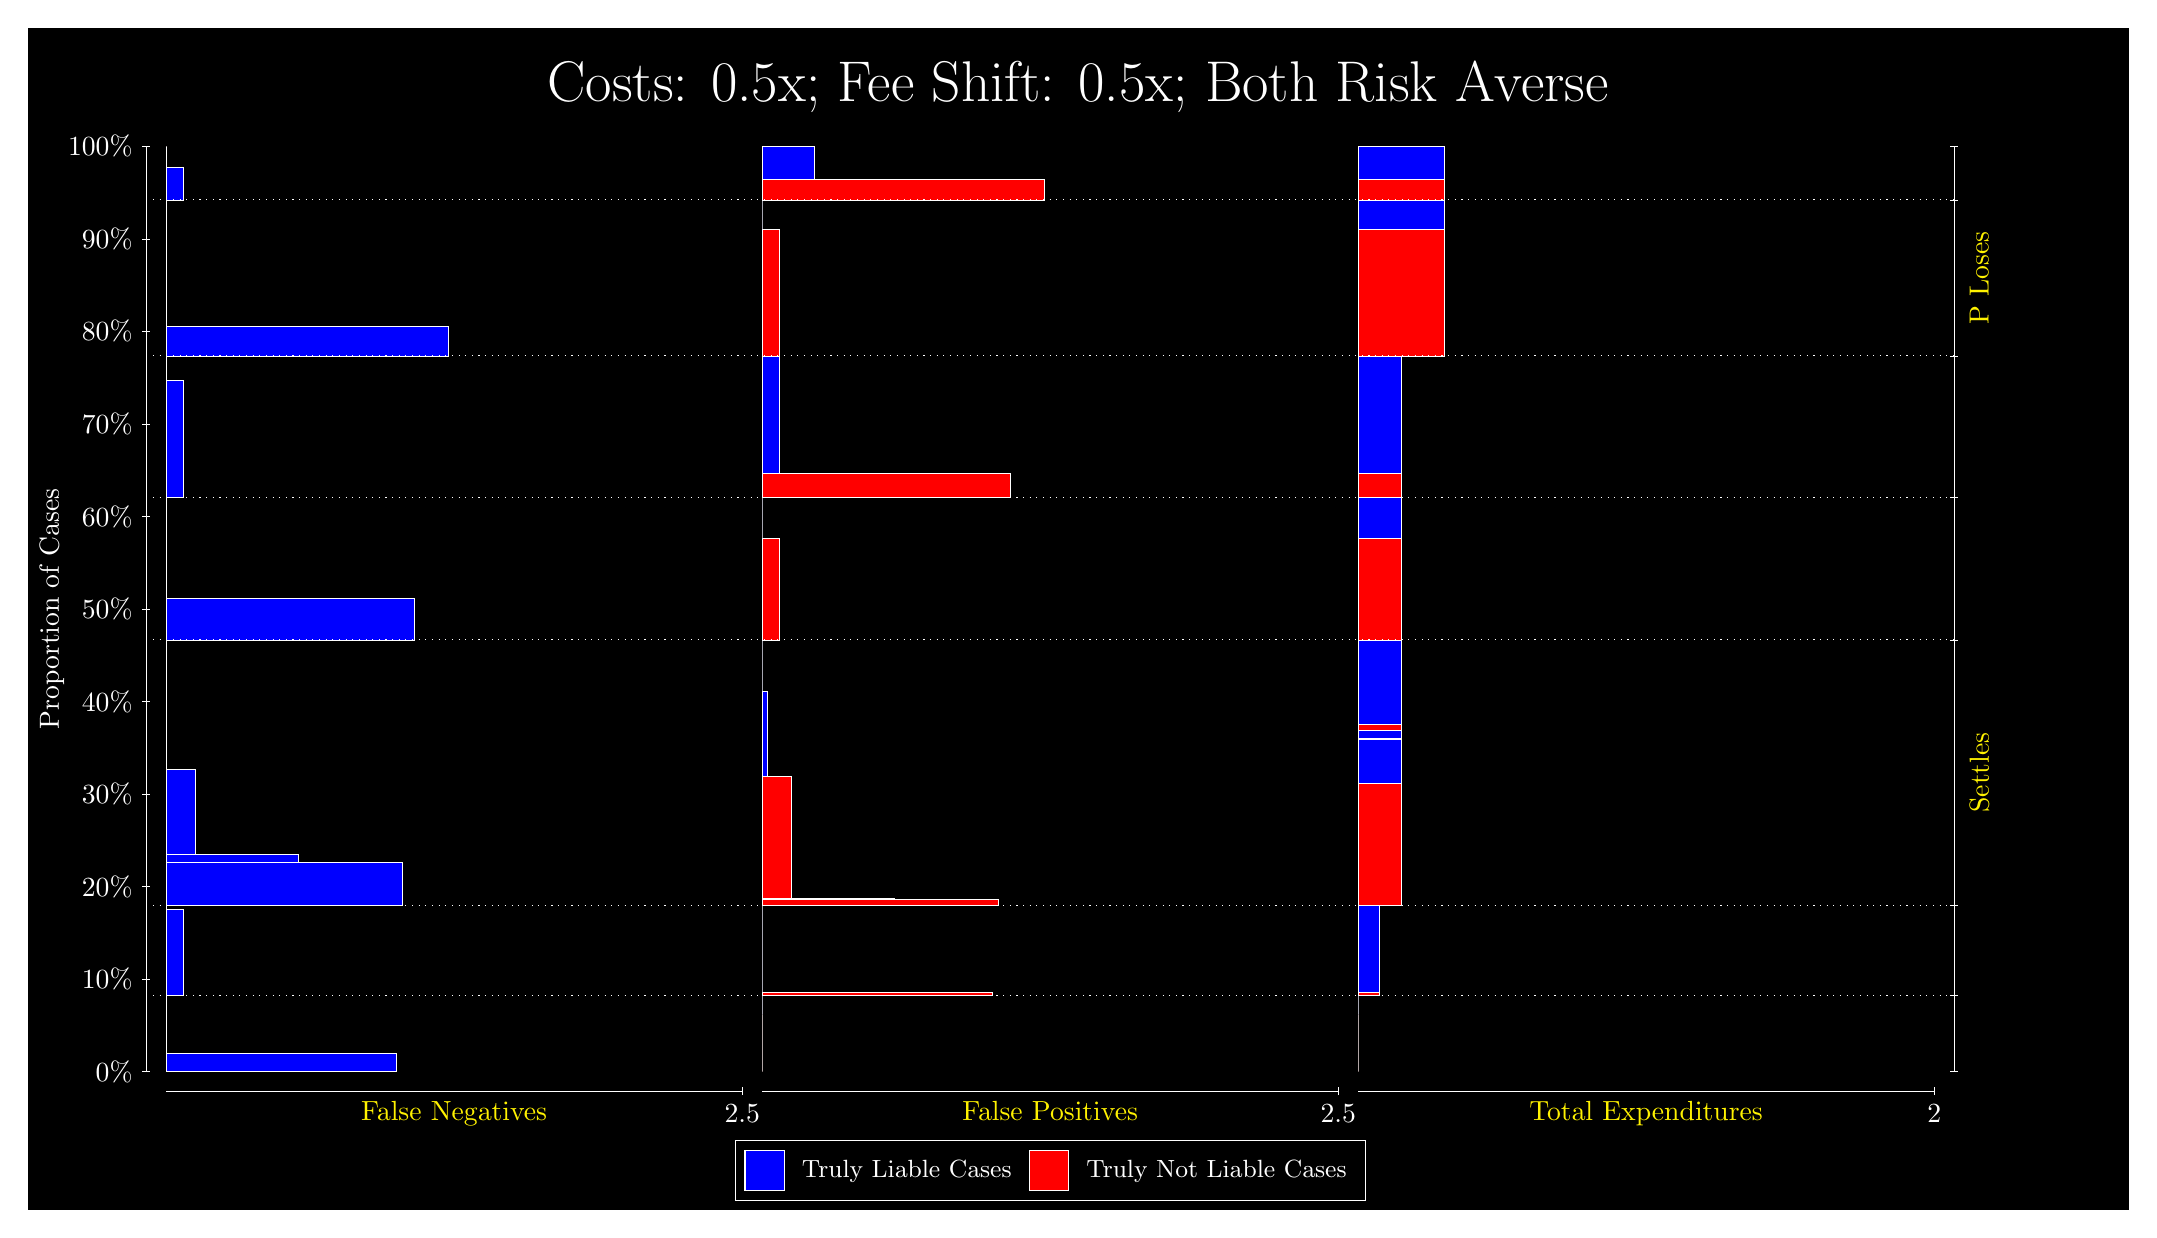
\begin{tikzpicture}
\draw[fill=black] (0,0) rectangle (26.667,15);
\draw[text=white] (0,13.5) rectangle (26.667,15) node[midway] {\huge Costs: 0.5x; Fee Shift: 0.5x; Both Risk Averse};
\draw[white, very thin] (1.5,1.75) -- (1.5,13.5);
\node[rotate=90, text=white, anchor=center] at (0.3, 7.625) {Proportion of Cases};
\draw[white, very thin] (1.45,1.75) -- (1.55,1.75);
\node[text=white, anchor=east] at (1.45, 1.75) {0\%};
\draw[white, very thin] (1.45,2.925) -- (1.55,2.925);
\node[text=white, anchor=east] at (1.45, 2.925) {10\%};
\draw[white, very thin] (1.45,4.1) -- (1.55,4.1);
\node[text=white, anchor=east] at (1.45, 4.1) {20\%};
\draw[white, very thin] (1.45,5.275) -- (1.55,5.275);
\node[text=white, anchor=east] at (1.45, 5.275) {30\%};
\draw[white, very thin] (1.45,6.45) -- (1.55,6.45);
\node[text=white, anchor=east] at (1.45, 6.45) {40\%};
\draw[white, very thin] (1.45,7.625) -- (1.55,7.625);
\node[text=white, anchor=east] at (1.45, 7.625) {50\%};
\draw[white, very thin] (1.45,8.8) -- (1.55,8.8);
\node[text=white, anchor=east] at (1.45, 8.8) {60\%};
\draw[white, very thin] (1.45,9.975) -- (1.55,9.975);
\node[text=white, anchor=east] at (1.45, 9.975) {70\%};
\draw[white, very thin] (1.45,11.15) -- (1.55,11.15);
\node[text=white, anchor=east] at (1.45, 11.15) {80\%};
\draw[white, very thin] (1.45,12.325) -- (1.55,12.325);
\node[text=white, anchor=east] at (1.45, 12.325) {90\%};
\draw[white, very thin] (1.45,13.5) -- (1.55,13.5);
\node[text=white, anchor=east] at (1.45, 13.5) {100\%};

\draw[white, very thin] (24.457,1.75) -- (24.457,13.5);
\draw[white, very thin] (24.407,1.75) -- (24.507,1.75);
\node[anchor=west] at (24.407, 1.75) {};
\draw[white, very thin] (24.407,2.7137) -- (24.507,2.7137);
\node[anchor=west] at (24.407, 2.7137) {};
\draw[white, very thin] (24.407,3.8608) -- (24.507,3.8608);
\node[anchor=west] at (24.407, 3.8608) {};
\draw[white, very thin] (24.407,7.2329) -- (24.507,7.2329);
\node[anchor=west] at (24.407, 7.2329) {};
\draw[white, very thin] (24.407,9.0435) -- (24.507,9.0435);
\node[anchor=west] at (24.407, 9.0435) {};
\draw[white, very thin] (24.407,10.839) -- (24.507,10.839);
\node[anchor=west] at (24.407, 10.839) {};
\draw[white, very thin] (24.407,12.82) -- (24.507,12.82);
\node[anchor=west] at (24.407, 12.82) {};
\draw[white, very thin] (24.407,13.5) -- (24.507,13.5);
\node[anchor=west] at (24.407, 13.5) {};

\draw[white, very thin, fill=blue] (1.75,1.75) rectangle (4.6775,1.9863);
\draw[white, very thin, fill=red] (1.75,1.9863) rectangle (1.75,2.7137);
\draw[white, very thin, fill=blue] (1.75,2.7137) rectangle (1.9696,3.8142);
\draw[white, very thin, fill=red] (1.75,3.8142) rectangle (1.75,3.8608);
\draw[white, very thin, fill=blue] (1.75,3.8608) rectangle (4.7507,4.4108);
\draw[white, very thin, fill=blue] (1.75,4.4108) rectangle (3.4333,4.5145);
\draw[white, very thin, fill=blue] (1.75,4.5145) rectangle (2.1159,5.592);
\draw[white, very thin, fill=red] (1.75,5.592) rectangle (1.75,7.2329);
\draw[white, very thin, fill=blue] (1.75,7.2329) rectangle (4.8971,7.7556);
\draw[white, very thin, fill=red] (1.75,7.7556) rectangle (1.75,9.0435);
\draw[white, very thin, fill=blue] (1.75,9.0435) rectangle (1.9696,10.534);
\draw[white, very thin, fill=red] (1.75,10.534) rectangle (1.75,10.839);
\draw[white, very thin, fill=blue] (1.75,10.839) rectangle (5.3362,11.215);
\draw[white, very thin, fill=red] (1.75,11.215) rectangle (1.75,12.82);
\draw[white, very thin, fill=blue] (1.75,12.82) rectangle (1.9696,13.238);
\draw[white, very thin, fill=red] (1.75,13.238) rectangle (1.75,13.5);
\draw[white, very thin, fill=red] (9.3189,1.75) rectangle (9.3189,2.4774);
\draw[white, very thin, fill=blue] (9.3189,2.4774) rectangle (9.3189,2.7137);
\draw[white, very thin, fill=red] (9.3189,2.7137) rectangle (12.246,2.7603);
\draw[white, very thin, fill=blue] (9.3189,2.7603) rectangle (9.3189,3.8608);
\draw[white, very thin, fill=red] (9.3189,3.8608) rectangle (12.32,3.9365);
\draw[white, very thin, fill=red] (9.3189,3.9365) rectangle (11.002,3.9456);
\draw[white, very thin, fill=red] (9.3189,3.9456) rectangle (9.6848,5.5017);
\draw[white, very thin, fill=blue] (9.3189,5.5017) rectangle (9.3921,6.5792);
\draw[white, very thin, fill=blue] (9.3189,6.5792) rectangle (9.3189,7.2329);
\draw[white, very thin, fill=red] (9.3189,7.2329) rectangle (9.5384,8.5208);
\draw[white, very thin, fill=blue] (9.3189,8.5208) rectangle (9.3189,9.0435);
\draw[white, very thin, fill=red] (9.3189,9.0435) rectangle (12.466,9.349);
\draw[white, very thin, fill=blue] (9.3189,9.349) rectangle (9.5384,10.839);
\draw[white, very thin, fill=red] (9.3189,10.839) rectangle (9.5384,12.444);
\draw[white, very thin, fill=blue] (9.3189,12.444) rectangle (9.3189,12.82);
\draw[white, very thin, fill=red] (9.3189,12.82) rectangle (12.905,13.082);
\draw[white, very thin, fill=blue] (9.3189,13.082) rectangle (9.9776,13.5);
\draw[white, very thin, fill=red] (16.888,1.75) rectangle (16.888,2.4774);
\draw[white, very thin, fill=blue] (16.888,2.4774) rectangle (16.888,2.7137);
\draw[white, very thin, fill=red] (16.888,2.7137) rectangle (17.162,2.7603);
\draw[white, very thin, fill=blue] (16.888,2.7603) rectangle (17.162,3.8608);
\draw[white, very thin, fill=red] (16.888,3.8608) rectangle (17.437,5.4169);
\draw[white, very thin, fill=blue] (16.888,5.4169) rectangle (17.437,5.967);
\draw[white, very thin, fill=red] (16.888,5.967) rectangle (17.437,5.976);
\draw[white, very thin, fill=blue] (16.888,5.976) rectangle (17.437,6.0796);
\draw[white, very thin, fill=red] (16.888,6.0796) rectangle (17.437,6.1554);
\draw[white, very thin, fill=blue] (16.888,6.1554) rectangle (17.437,7.2329);
\draw[white, very thin, fill=red] (16.888,7.2329) rectangle (17.437,8.5208);
\draw[white, very thin, fill=blue] (16.888,8.5208) rectangle (17.437,9.0435);
\draw[white, very thin, fill=red] (16.888,9.0435) rectangle (17.437,9.349);
\draw[white, very thin, fill=blue] (16.888,9.349) rectangle (17.437,10.839);
\draw[white, very thin, fill=red] (16.888,10.839) rectangle (17.986,12.444);
\draw[white, very thin, fill=blue] (16.888,12.444) rectangle (17.986,12.82);
\draw[white, very thin, fill=red] (16.888,12.82) rectangle (17.986,13.082);
\draw[white, very thin, fill=blue] (16.888,13.082) rectangle (17.986,13.5);
\draw[white, dotted] (1.5,2.7137) -- (24.457,2.7137);
\draw[white, dotted] (1.5,3.8608) -- (24.457,3.8608);
\draw[white, dotted] (1.5,7.2329) -- (24.457,7.2329);
\draw[white, dotted] (1.5,9.0435) -- (24.457,9.0435);
\draw[white, dotted] (1.5,10.839) -- (24.457,10.839);
\draw[white, dotted] (1.5,12.82) -- (24.457,12.82);
\draw[white, very thin] (1.75,1.5) -- (9.0689,1.5);
\node[text=yellow, anchor=north] at (5.4094, 1.5) {False Negatives};
\draw[white, very thin] (9.0689,1.45) -- (9.0689,1.55);
\node[text=white, anchor=north] at (9.0689, 1.45) {2.5};

\draw[white, very thin] (9.3189,1.5) -- (16.638,1.5);
\node[text=yellow, anchor=north] at (12.978, 1.5) {False Positives};
\draw[white, very thin] (16.638,1.45) -- (16.638,1.55);
\node[text=white, anchor=north] at (16.638, 1.45) {2.5};

\draw[white, very thin] (16.888,1.5) -- (24.207,1.5);
\node[text=yellow, anchor=north] at (20.547, 1.5) {Total Expenditures};
\draw[white, very thin] (24.207,1.45) -- (24.207,1.55);
\node[text=white, anchor=north] at (24.207, 1.45) {2};



\node[text=yellow, centered, rotate=90] at (24.777, 5.5468) {Settles};


\node[text=yellow, centered, rotate=90] at (24.777, 11.83) {P Loses};


\draw (12.978300999999998,1.5) node[draw=none] (baseCoordinate) {};
\begin{scope}[align=center]
        \matrix[scale=0.5, draw=white, below=0.5cm of baseCoordinate, nodes={draw}, column sep=0.1cm]{
            \node[rectangle, draw, minimum width=0.5cm, minimum height=0.5cm, fill=blue] {}; &
            \node[draw=none, font=\small, text=white] (B) {Truly Liable Cases}; &
            \node[rectangle, draw, minimum width=0.5cm, minimum height=0.5cm, fill=red] {}; &
            \node[draw=none, font=\small, text=white] (B) {Truly Not Liable Cases}; \\
            };
\end{scope}

\end{tikzpicture}
\end{document}